% ドキュメントの設定
\documentclass[a4paper,11pt,xelatex,ja=standard]{bxjsarticle}
\usepackage{tikz}
\usetikzlibrary {datavisualization.formats.functions}
\usepackage{pgfplots}
\usepackage{float}

% ドキュメント開始
\begin{document}

\section{実験の目的}

    トランジスタによって信号を適切に増幅するためにはバイアスの設定が重要となる。本実験では電界効果トランジスタのバイアス方法とソース接地増幅回路の基本特性を習得する。

\section{実験の理論または原理}
    \subsection{バイアス回路}
        トランジスタを動作させるために加える直流電圧を「バイアス電圧」といって,バイアスとして与える直流電流を「バイアス電流」と呼ぶ。適切に増幅された信号をトランジスタから得るためにはバイアスが必要になる。このバイアスを与える回路がバイアス回路であり,用途によっていくつかの回路が使い分けられている。
        \subsubsection{固定バイアス回路}
            固定バイアス回路では,ドレイン・ソース間電圧$V_{DS}$を与える電源$V_{DD}$に加えて,ゲート・ソース間電圧$V_{GS}$を与える電源$V_G$を別に設けて動作点を決定する。動作点はドレイン電流$I_D$の変化に対して変わらないため,電力増幅などのドレイン電流$I_D$が大きく変化する回路に用いられる。
        \subsubsection{自己バイアス回路}
            FETが小信号用として使われるときには,出力交流信号$d_i$の振幅がそれほど大きくないので,ドレイン電流$I_D$はほぼ一定とみなせる。そこで,ソースに直列に抵抗$R_S$を接続するとその電圧降下をバイアスとして利用することができる。これを自己バイアス回路と呼ぶ。自己バイアス回路では,何らかの原因でドレイン電流$I_D$が増加しても,ゲート・ソース間電圧$V_{GS}$が$I_D \times R_S$ によって決定されるため$(V_{GS} = - R_S I_D)$,$V_{GS}$がマイナス方向に増加して$I_D$の増加を抑える方向に働く。一方,$I_D$が減少すると$V_{GS}$が減少して,$I_D$の減少を抑える方向に働く。よって,自己バイアス回路は動作点の変動を防ぐように働くので小信号増幅回路では良く用いられる。一方,電力増幅回路のように$I_D$が大きく変化する回路に用いると,$I_D$の変化を抑えるように働くため不都合が生じてしまう。
        \subsubsection{固定バイアス法と自己バイアス法を併用する方式}
            このバイアス方法は,固定バイアス法と自己バイアス法を併用したもので,両者の長所を兼ね備えたバイアス法で,一般的に使用されている。
        \subsubsection{固定バイアス法と自己バイアス法を併用する方式}
            バイアス回路における電圧と電流の関係

            \begin{enumerate}
                \item[(a)] ゲート・ソース間電圧\( V_{GS} \)とドレイン電流\( I_D \)との関係
                \[ I_D = I_{DSS} \left( 1 - \frac{V_{GS}}{V_P} \right)^2 \quad (1) \]
            
                \item[(b)] ゲート電圧\( V_G \)と\( R_1 \),\( R_2 \)(ブリーダ抵抗と呼ばれる)との関係
                \[ V_G = \frac{R_1}{R_1 + R_2} V_{DD} \quad (2) \]
            
                \item[(c)] ゲート・ソース間電圧\( V_{GS} \)とソース抵抗\( R_S \)の関係
                \[ V_{GS} = V_G - I_D R_S \quad (3) \]
                ゲート電圧に\( I_D R_S \)という電圧がフィードバックされ,安定度が改善される。
            
                \item[(d)] ソース抵抗\( R_S \)とドレイン電流\( I_D \)との関係
                \[ R_s = \frac{1 - \left( \frac{I_D}{I_{DSS}} \right) ^{\frac{1}{2}}}{I_D} \]

            \end{enumerate}
    \subsection{基本増幅回路}
        FET を使用する場合,その接地方式および出力の取り出し方により,次の3つに分類できる。
        \subsubsection{ソース接地増幅回路}
            ソース接地増幅回路は高入力インピーダンス,電圧利得を大きくできるといった特徴があり,良く用いられる回路である。
            \begin{enumerate}
                \item[(a)] 入力信号電圧$i_v$とすると,ドレイン電流の交流分$D_i$は次のように表される。
                    \[ i_D = g_m V_i \]
                \item[(b)] 出力電圧の交流分$o_v$は次式で表される。
                    \[ v_o = - i_D R_L = - g_m v_i R_L \]
                \item[(c)] 電圧増幅度$v_A$は次式で与えられる。
                    \[ A_v = \frac{V_o}{V_i} = - g_m R_L \]
            \end{enumerate}
        \subsubsection{ドレイン接地増幅回路(ソース・フォロア増幅回路)}
            ドレイン接地増幅回路は電圧利得が1以上になることはないが,高入力インピーダンスで入力信号を取り入れて,低出力インピーダンスで信号を送り出す,インピーダンス変換回路として用いられる。
        \subsubsection{ゲート接地増幅回路}
            この方式の場合には,電圧利得はソース接地の場合と同じであるが,入力インピーダンスを小さくできる。この場合,トランジスタでもよいが,高周波での安定な増幅に利点がある。
    
\section{実験の作業順序}
    回路におけるバイアス条件は次の2種類とする。

    \subsubsection*{バイアス条件1}
    \begin{itemize}
        \item $R_1 = 33$ k$\Omega$
        \item $R_2 = 56$ k$\Omega$
        \item $R_L = 2.2$ k$\Omega$
        \item $R_S = 4.7$ k$\Omega$
    \end{itemize}

    
    \subsection*{バイアス条件2}
    \begin{itemize}
        \item $R_1 = 11$ k$\Omega$
        \item $R_2 = 120$ k$\Omega$
        \item $R_L = 4.7$ k$\Omega$
        \item $R_S = 2.2$ k$\Omega$
    \end{itemize}
    
    \begin{figure}[H]
        \centering
        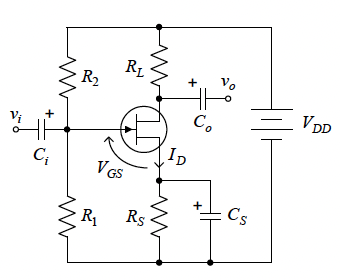
\includegraphics[width=0.5\textwidth]{./img/4/pic-1.png}
        \caption{回路図}
    \end{figure}

    \subsection{ソース接地増幅回路におけるバイアス電圧の設定と測定}
        \begin{enumerate}
            \item バイアス条件1の回路構成での各抵抗における電圧値$V_{R1},V_{R2},V_{RL},V_{RS}$を計算する。
            \item 配線後,直流電圧を印加して$V_{R1}$,$V_{R2}$,$V_{RL}$,$V_{RS}$を測定する。さらに,ドレイン・ソース間電圧VDS,ゲート・ソース間電圧$V_{GS}$を測定する。
        \end{enumerate}
    
    \subsection{ソース接地増幅回路におけるバイアス電圧の設定と測定}
        \begin{enumerate}
            \item 入力信号$i_v$ を設定する。周波数をf=10[kHz]として,オシロスコープで入力信号波形を観測しながら振幅を50[mV]程度に設定する。このとき,入力信号の波形が歪まない電圧値に設定すること。
            \item 入力信号の周波数を10[Hz]~1000[kHz]まで変化させ、その時の入力電圧iv と出力電圧ov を測定する。このとき、入力信号の振幅を一定に保つように注意すること。また、周波数の測定間隔はグラフを描きながら適切に設定すること。
            \item 増幅度$v_A$[倍]を電圧利得$v_G$[dB]で表示する。
                \[G_v = 20 \log A_v = 20 \log \frac{V_o}{V_i}\]
        \end{enumerate}

\section{実験の結果}
    \subsubsection{ドレイン接地増幅回路(ソース・フォロア増幅回路)}
        % 条件1トランジスタ1
        \begin{figure}[H]
            \centering
            \begin{tikzpicture}[scale=0.9]
                \datavisualization[ 
                    scientific axes,
                    visualize as line/.list={index_a, index_b}, 
                    index_a={style={thick,mark=*,black},label in legend={text=入力}},
                    index_b={style={thick,dashed,mark=triangle,black},label in legend={text=出力}},
                    legend={north west outside},
                    x axis={logarithmic,label={周波数[Hz]},length=10cm},
                    y axis={label={電圧[mV]},length=6cm,min value=0, max value=320},
                ]
                data[set=index_a] {
                    x, y
                    10,50.4
                    20,51.2
                    30,56
                    40,53.6
                    50,58.4
                    70,49.6
                    100,54.4
                    200,50.4
                    300,54.4
                    400,52
                    500,56.8
                    700,51.2
                    1000,51.2
                    2000,51.2
                    3000,52.8
                    4000,50.4
                    5000,54.4
                    7000,52
                    10000,55.2
                    20000,56.8
                    30000,49.6
                    40000,53.6
                    50000,52.8
                    70000,52.8
                    100000,52.8
                    200000,53.6
                    300000,52
                    400000,48.8
                    500000,48
                    700000,48.8
                    1000000,47.2
                }
                data[set=index_b] {
                    x, y
                    10,72
                    20,112
                    30,138
                    40,126
                    50,164
                    70,176
                    100,180
                    200,192
                    300,192
                    400,196
                    500,192
                    700,188
                    1000,196
                    2000,192
                    3000,196
                    4000,196
                    5000,192
                    7000,200
                    10000,200
                    20000,196
                    30000,196
                    40000,196
                    50000,196
                    70000,200
                    100000,200
                    200000,196
                    300000,196
                    400000,196
                    500000,192
                    700000,188
                    1000000,180
                };
            \end{tikzpicture}
            \caption{条件1トランジスタ1}
        \end{figure} % merge

        % 条件2トランジスタ1
        \begin{figure}[H]
            \centering
            \begin{tikzpicture}[scale=0.9]
                \datavisualization[ 
                    scientific axes,
                    visualize as line/.list={index_a, index_b}, 
                    index_a={style={thick,mark=*,black},label in legend={text=入力}},
                    index_b={style={thick,dashed,mark=triangle,black},label in legend={text=出力}},
                    legend={north west outside},
                    x axis={logarithmic,label={周波数[Hz]},length=10cm},
                    y axis={label={電圧[mV]},length=6cm,min value=0, max value=450},
                ]
                data[set=index_a] {
                    x, y
                    10,48.8
                    20,49.6
                    30,49.6
                    40,49.6
                    50,49.6
                    70,48.8
                    100,49.6
                    200,49.6
                    300,50.4
                    400,49.6
                    500,50.4
                    700,50.4
                    1000,49.6
                    2000,49.6
                    3000,50.4
                    4000,49.6
                    5000,50.4
                    7000,50.4
                    10000,50.4
                    20000,50.4
                    30000,50.4
                    40000,50.4
                    50000,51.2
                    70000,51.2
                    100000,51.2
                    200000,50.4
                    300000,50.4
                    400000,51.2
                    500000,50.4
                    700000,49.6
                    1000000,50.4
                }
                data[set=index_b] {
                    x, y
                    10,168
                    20,232
                    30,288
                    40,312
                    50,336
                    70,360
                    100,384
                    200,392
                    300,400
                    400,400
                    500,408
                    700,408
                    1000,408
                    2000,408
                    3000,416
                    4000,416
                    5000,416
                    7000,416
                    10000,416
                    20000,424
                    30000,424
                    40000,416
                    50000,416
                    70000,424
                    100000,424
                    200000,424
                    300000,416
                    400000,408
                    500000,392
                    700000,376
                    1000000,352
                };
            \end{tikzpicture}
            \caption{条件2トランジスタ1}
        \end{figure}

        % 条件1トランジスタ2
        \begin{figure}[H]
            \centering
            \begin{tikzpicture}[scale=0.9]
                \datavisualization[ 
                    scientific axes,
                    visualize as line/.list={index_a, index_b}, 
                    index_a={style={thick,mark=*,black},label in legend={text=入力}},
                    index_b={style={thick,dashed,mark=triangle,black},label in legend={text=出力}},
                    legend={north west outside},
                    x axis={logarithmic,label={周波数[Hz]},length=10cm},
                    y axis={label={電圧[mV]},length=6cm,min value=0, max value=320},
                ]
                data[set=index_a] {
                    x, y
                    10,56.8
                    20,50.4
                    30,51.2
                    40,52.8
                    50,55.2
                    70,52.8
                    100,51.2
                    200,57.6
                    300,56
                    400,52
                    500,56
                    700,55.2
                    1000,56
                    2000,50.4
                    3000,52.8
                    4000,51.2
                    5000,53.6
                    7000,51.2
                    10000,56
                    20000,52.8
                    30000,52
                    40000,52.8
                    50000,53.6
                    70000,52
                    100000,53.6
                    200000,55.2
                    300000,49.6
                    400000,48.8
                    500000,49.6
                    700000,52
                    1000000,48.8
                }
                data[set=index_b] {
                    x, y
                    10,90
                    20,102
                    30,134
                    40,158
                    50,180
                    70,212
                    100,264
                    200,280
                    300,286
                    400,288
                    500,288
                    700,288
                    1000,290
                    2000,292
                    3000,292
                    4000,292
                    5000,294
                    7000,294
                    10000,296
                    20000,296
                    30000,298
                    40000,298
                    50000,296
                    70000,298
                    100000,300
                    200000,296
                    300000,294
                    400000,290
                    500000,290
                    700000,282
                    1000000,270
                };
            \end{tikzpicture}
            \caption{条件1トランジスタ2}
        \end{figure}

        % 条件2トランジスタ2
        \begin{figure}[H]
            \centering
            \begin{tikzpicture}[scale=0.9]
                \datavisualization[ 
                    scientific axes,
                    visualize as line/.list={index_a, index_b}, 
                    index_a={style={thick,mark=*,black},label in legend={text=入力}},
                    index_b={style={thick,dashed,mark=triangle,black},label in legend={text=出力}},
                    legend={north west outside},
                    x axis={logarithmic,label={周波数[Hz]},length=10cm},
                    y axis={label={電圧[mV]},length=6cm,min value=0, max value=500},
                ]
                data[set=index_a] {
                    x, y
                    10,44
                    20,49.6
                    30,42.4
                    40,45.6
                    50,48.8
                    70,44
                    100,44.8
                    200,46.4
                    300,44.8
                    400,44
                    500,46.4
                    700,48
                    1000,44.8
                    2000,46.4
                    3000,48
                    4000,45.6
                    5000,47.2
                    7000,50.4
                    10000,48
                    20000,48
                    30000,48
                    40000,46.4
                    50000,48.8
                    70000,46.4
                    100000,44
                    200000,46.4
                    300000,44.4
                    400000,45.6
                    500000,42.4
                    700000,44.8
                    1000000,44
                }
                data[set=index_b] {
                    x, y
                    10,152
                    20,224
                    30,288
                    40,328
                    50,356
                    70,392
                    100,412
                    200,440
                    300,444
                    400,444
                    500,448
                    700,452
                    1000,448
                    2000,452
                    3000,456
                    4000,456
                    5000,456
                    7000,452
                    10000,460
                    20000,456
                    30000,464
                    40000,464
                    50000,460
                    70000,460
                    100000,460
                    200000,456
                    300000,440
                    400000,436
                    500000,424
                    700000,404
                    1000000,364
                };
            \end{tikzpicture}
            \caption{条件2トランジスタ2}
        \end{figure}

\section{実験の考察およびまとめ}

\end{document}